\chapter{Mask Post-Processing Techniques}\label{ch:postProcessing}

As shown in Chapter \ref{ch:cetDet}, at this stage the Mask R-CNN model is capable of detecting cetaceans at an individual pixel level. Before these detections can be passed to the identification module, some post-processing of the output must be performed to allow for both a reduction in the computational expense of operating on the detector's output as well as ensuring that no potentially important information which will assist in an identification is lost. As such, the following chapter details the mask post-processing techniques implemented as required by the system pipeline, as shown in Figure \ref{fig:pipeline-post-processed}.

\begin{figure}[!h]
	\begin{center}
		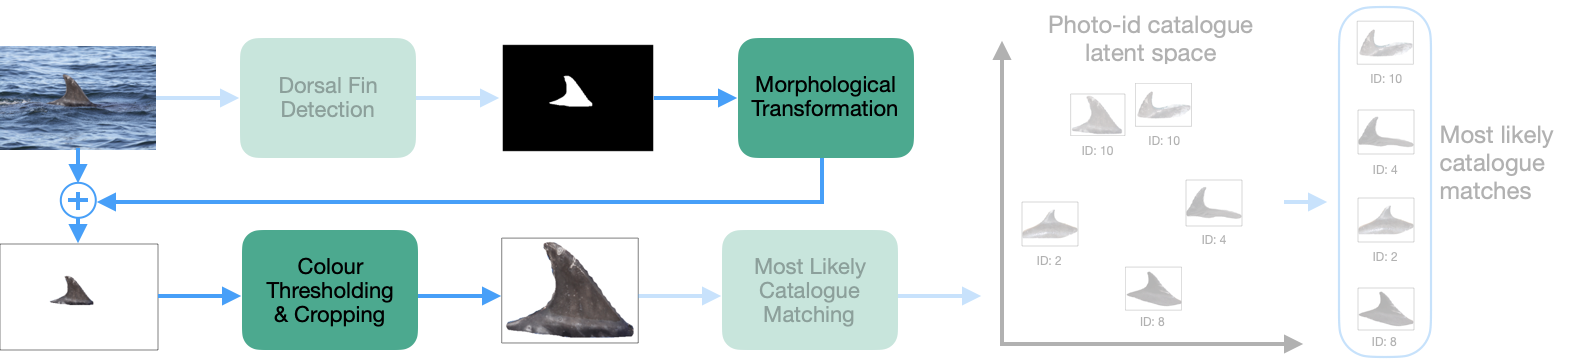
\includegraphics[width=\linewidth]{Chapter5/figs/pipeline-post-processed.png}
	\end{center}
	\caption[The high level pipeline overview, shown in Figure \ref{fig:pipeline}, with the post-processing techniques highlighted.]{The high level pipeline overview, shown in Figure \ref{fig:pipeline}, with the post-processing techniques highlighted. It is this part of the pipeline that will be discussed in the following section.}
	\label{fig:pipeline-post-processed}
\end{figure}

\section{Handling Multiple Detections}\label{ch:postProcessing,sec:handlingMultipleDetections}

When an image is passed through the Mask R-CNN detector, the number of outputs can vary depending on how many detected objects have a confidence score higher than 90\% (as discussed in Section \ref{ch:cetDet,sec:ModelSelection,sub:DetectionHyperparameters}). If no detections reach this threshold the image is discarded from further processing. This can occur if, for example, an image is taken by accident capturing the vessel's floor. If a single detection reaches the threshold, the resultant mask is passed downstream. 

Thanks to the tendency for cetaceans to travel in pods however, it is unlikely an image will contain only a single \texttt{dolphin} detection. In these situations the Mask R-CNN will output multiple detection masks, one per object. To handle this, the first stage of the post-processing methodology is to separate multiple detections for a single image. This ensures each \texttt{dolphin} detection is handled independently, mitigating the potential for an identification to be influenced by the others. An example of this behaviour can be seen in Figure \ref{fig:190730-001-MOLS0360_-detections}. Here, an image inputted to the Mask R-CNN detector has produced three detections which are above the threshold. As such, they have been split into three output masks for individual processing. Note that the first detected mask, visualised with a blue overlay on the input image, has been incorrectly detected as \texttt{dolphin} with a high confidence resulting in a binary mask. Further post-processing must be capable of handling background which has been incorrectly labelled, removing it before individual identification occurs.

\begin{figure}
	\begin{center}
		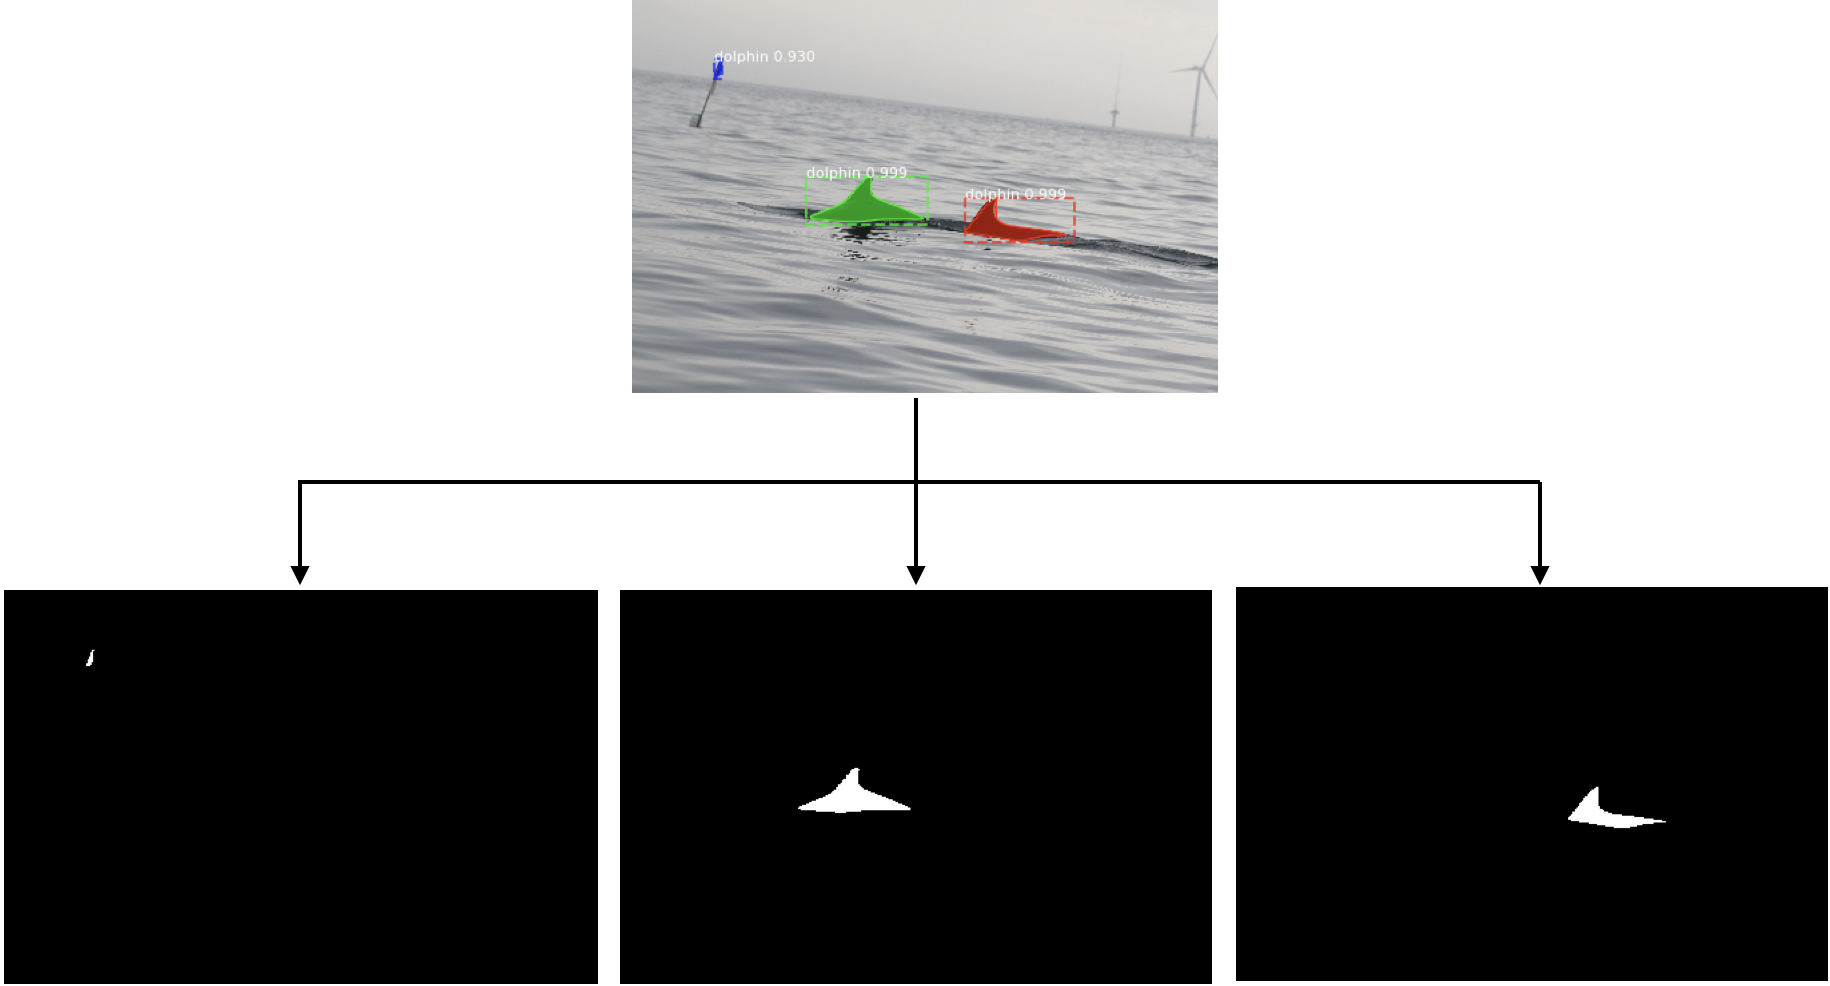
\includegraphics[scale=0.45]{Chapter5/figs/190730-001-MOLS0360_-detections.png}
	\end{center}
	\caption[A visualisation of the three \texttt{dolphin} detections for an input image produced by the Mask R-CNN detector.]{A visualisation of the three \texttt{dolphin} detections for an input image produced by the Mask R-CNN detector. The detections are highlighted by the blue, green, and red overlays on the input image, top. The resultant detection masks once split are shown bottom, where a \texttt{dolphin} object is displayed in white.}
	\label{fig:190730-001-MOLS0360_-detections}
\end{figure}

\section{Morphological Transformations}\label{ch:postProcessing,sec:morphologicalTransformations}

In some situations a detected mask may contain an area of background inside the detection. This can be thought of as a hole in the detection, as seen in Figure \ref{fig:before-and-after-morphing-masks-only} (Left). Using \textit{a priori} knowledge of cetaceans, which would rarely if ever be captured with a hole, it can be deduced that a hole in the detection is highly unlikely and may cause a loss of useful identifying information. As such, any holes which are present in the masks must be filled.  

\begin{figure}
	\begin{center}
		
\includegraphics[scale=0.5]{Chapter5/figs/before-and-after-morphing-masks-only.png}
	\end{center}
	\caption[Left: a detection mask before closing has been applied. Right: the same detection mask after closing.]{Left: a detection mask before closing has been applied. The detected \texttt{dolphin} object is displayed in white. Note the cluster of black background pixels inside. Right: the same detection mask after closing. Note the pixels which make up the hole have been converted to \texttt{dolphin}.}
	\label{fig:before-and-after-morphing-masks-only}
\end{figure}

This is achieved using morphological transformations, a set of operations which allow for the automated manipulation of the internal structure of binary images such as masks. The two fundamental morphological transformations are erosion, which erodes away the boundaries of the masked object, and dilation, which increases the size of the object by pushing the boundary out into the background space. These two operations can be utilised in various combinations to perform more complex transformations.

In order to remove a cluster of background pixels inside of a detection, each mask is closed -- dilated then eroded. This has the effect of removing any holes present inside the mask, as can be seen in Figure \ref{fig:before-and-after-morphing-masks-only} (Right). If no holes exist, the operation is still performed, however the mask remains unchanged. By performing closing, the system ensures that no potentially identifiable information is lost as a result of an incomplete detection. 

\section{Background Subtraction}\label{ch:postProcessing,sec:bgExtraction}

Now that the masks have been cleaned using morphological transformations, it is possible to utilise them to perform background subtraction. This is an extremely important step in producing an accurate individual classification based on the detected \texttt{dolphin} object by ensuring a minimal amount of background noise is passed to the identification system.

As both the input image and resultant mask can be represented as matrices, these can be manipulated utilising a \textit{bitwise and} operation such that if pixel$_{i, j}$ in the input image is denoted as background in the mask, the values of pixel$_{i, j}$ can be set to [255, 255, 255] (white). This has the effect of whiting out any pixels not detected as part of the \texttt{dolphin} in the input, whilst keeping the pixels detected as \texttt{dolphin} intact.

An example of background subtraction utilising cleaned masks can be seen in Figure \ref{fig:190730-001-MOLS0360_-bg-subtraction}. Using the same input image as in Figure \ref{fig:190730-001-MOLS0360_-detections}, it can be seen that the \textit{bitwise and} operation whites all pixels in the image except those which have been classified as \texttt{dolphin} for each of the three output masks. Note at this point that the erroneous classification still remains. 

\begin{figure}
	\begin{center}
		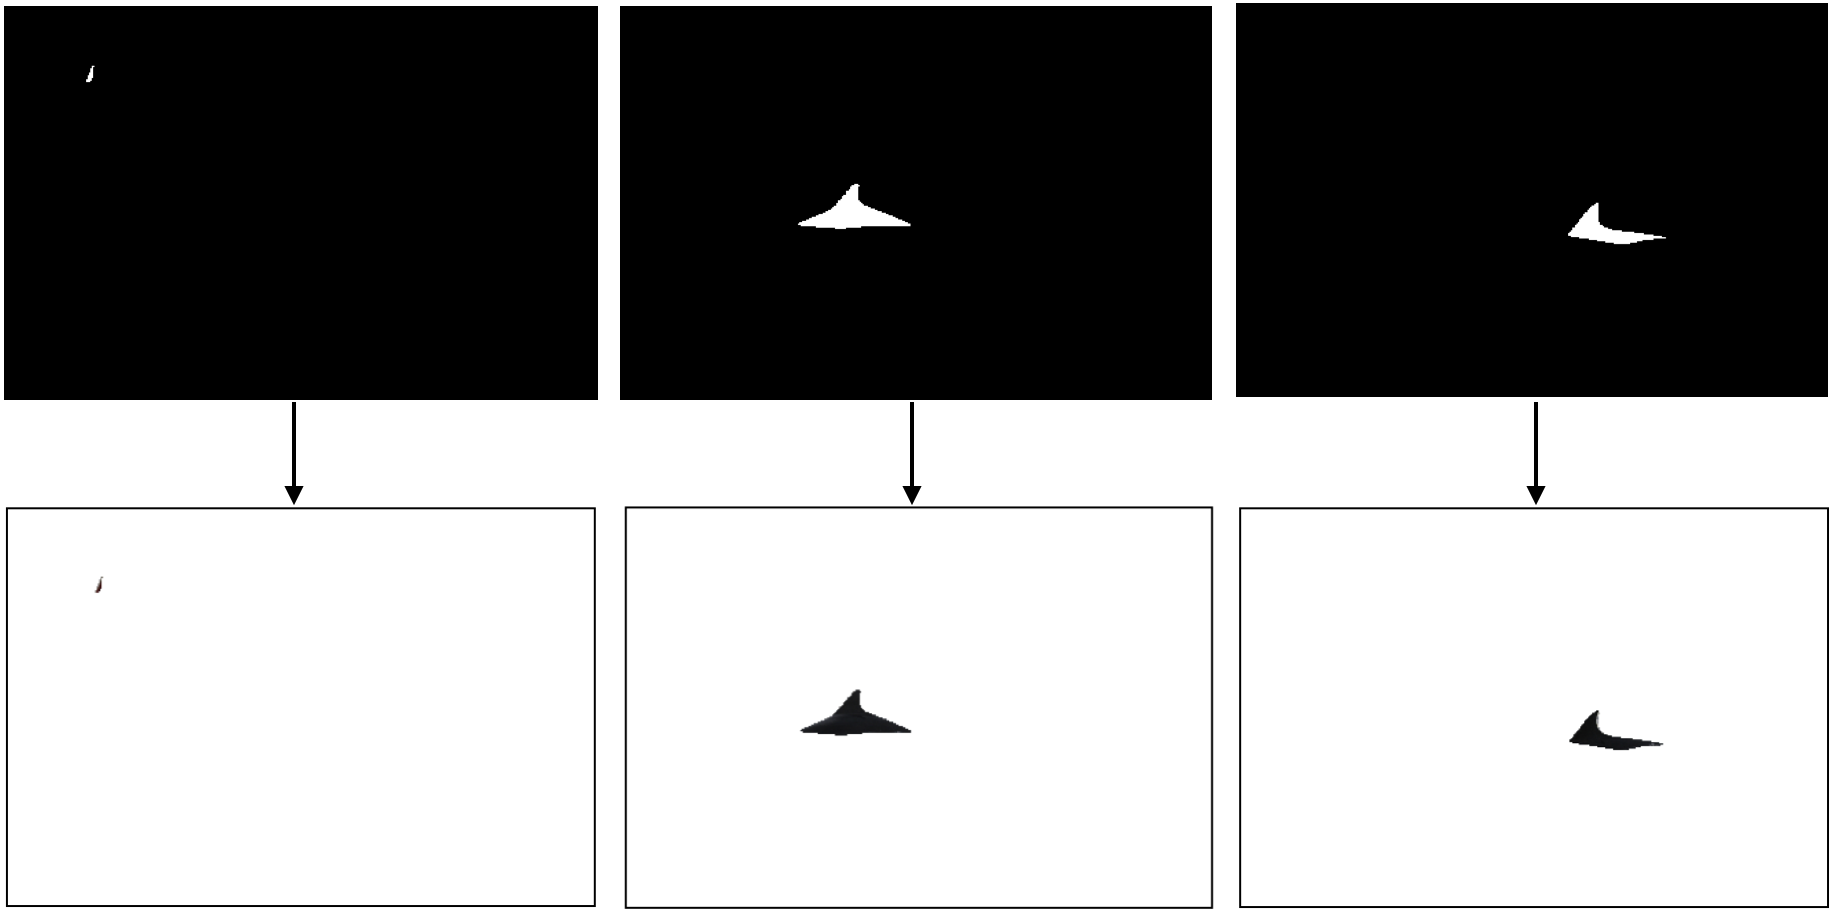
\includegraphics[scale=0.45]{Chapter5/figs/190730-001-MOLS0360_-bg-subtraction.png}
	\end{center}
	\caption[A visualisation of the three \texttt{dolphin} detections from Figure \ref{fig:190730-001-MOLS0360_-detections} before and after background subtraction.]{A visualisation of the three \texttt{dolphin} detections from Figure \ref{fig:190730-001-MOLS0360_-detections} before and after background subtraction. A border has been added to the background subtracted images for clarity.}
	\label{fig:190730-001-MOLS0360_-bg-subtraction}
\end{figure}

Whilst the background subtraction aims to reduce noise passed downstream to the individual identification module, it will not be possible to remove all noise. It may be the case, such as in Figure \ref{fig:fin-extraction-unclean}, that some background pixels are mislabelled as \texttt{dolphin} but are connected to the edges of a correct detection. As a result, morphological transformation and background subtraction are unable to remove the mislabelled pixels. This may affect the accuracy of identification downstream unless the system is robust enough to deal with this.

\begin{figure}
	\begin{center}
		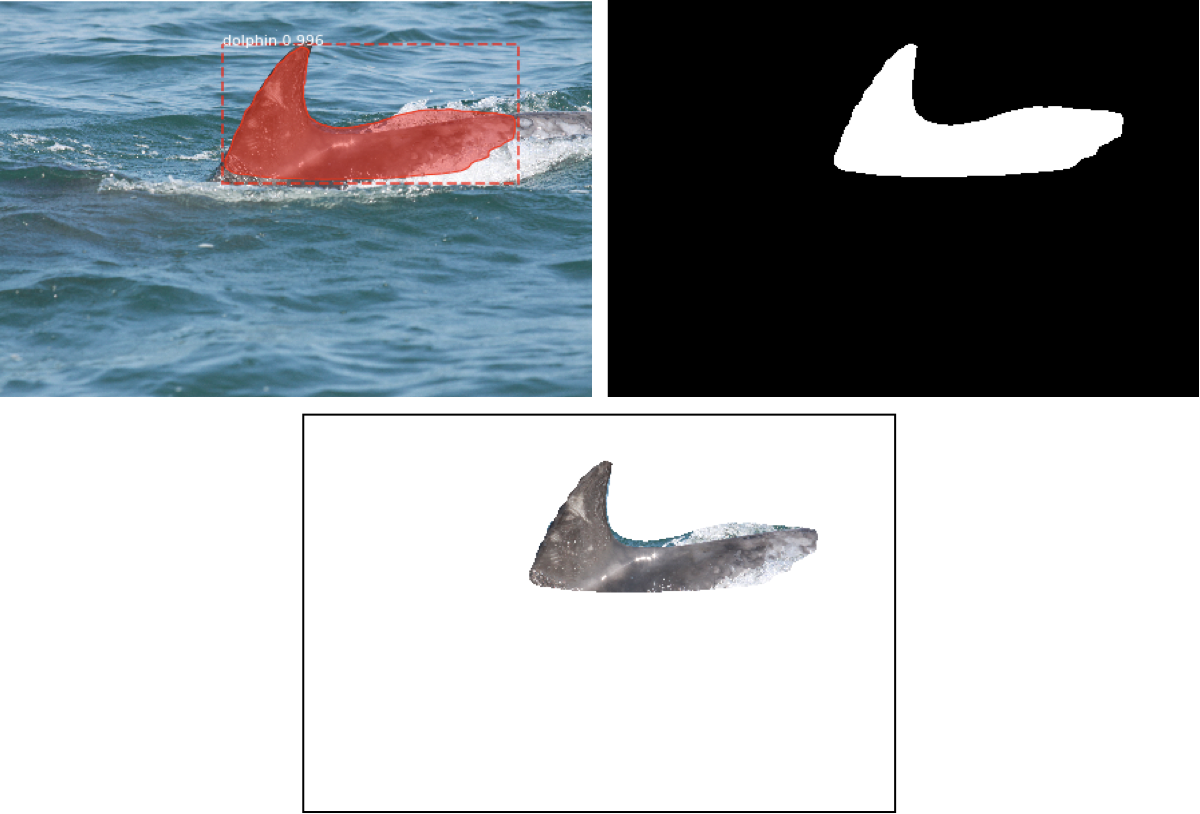
\includegraphics[scale=0.5]{Chapter5/figs/fin-extraction-unclean-uncropped.png}
	\end{center}
	\caption[Top Left: a visualisation of the \texttt{dolphin} detection for an input image produced by the Mask R-CNN detector, alongside the confidence score. Top Right: the resultant detection mask after morphological transformation. Bottom: the resultant output image after \textit{bitwise and} operations performed between the input image and the cleaned detection mask.]{Top Left: a visualisation of the \texttt{dolphin} detection for an input image produced by the Mask R-CNN detector, alongside the confidence score. The detector has incorrectly labelled some pixels as \texttt{dolphin}. Top Right: the resultant detection mask after morphological transformation. Bottom: the resultant output image after \textit{bitwise and} operations performed between the input image and the cleaned detection mask. Note the mislabelled pixels are present after cleaning and background subtraction. A border has been added for clarity.}
	\label{fig:fin-extraction-unclean}
\end{figure}

\section{Colour Thresholding Mask Components}\label{ch:postProcessing,sec:colourThresholdingMaskComponents}

In some cases a single detection mask may consist of multiple components. This may occur if, for example, an area of splash has been erroneously included as part of a detection. As cetaceans cannot be made up of multiple disjoint components, it is known that some of these must be noise and can be removed. 

The outer layer of a cetacean's skin is often a consistent grey colouring. This information can be utilised to filter out noisy components of the mask during post-processing. By comparing the colour composition of each detected object against a calculated \textit{dolphin-like} threshold, it is possible to discard mask components which have been erroneously detected.

In order to be able to compare each mask component's composition against a \textit{dolphin-like} colour threshold, the values of the threshold must first be determined. To achieve this, each image in the Zanzibar dataset was run through the Mask R-CNN detector. Histograms of the three RGB colour channel pixel intensities for each object classification (\texttt{dolphin} or background) were recorded, giving a total of six histograms per image. 

Once complete the histogram groups were combined to give six global pixel intensity distributions, which can be seen in Figure \ref{fig:global-histogram}. From the charts it can be seen that, regardless of colour channel, there is a near inversion in the distribution of pixel intensities between those detected as \texttt{dolphin} and those not, strongly suggesting it is possible to determine whether a component is erroneous based on its colour composition.

\begin{figure}
	\begin{center}
		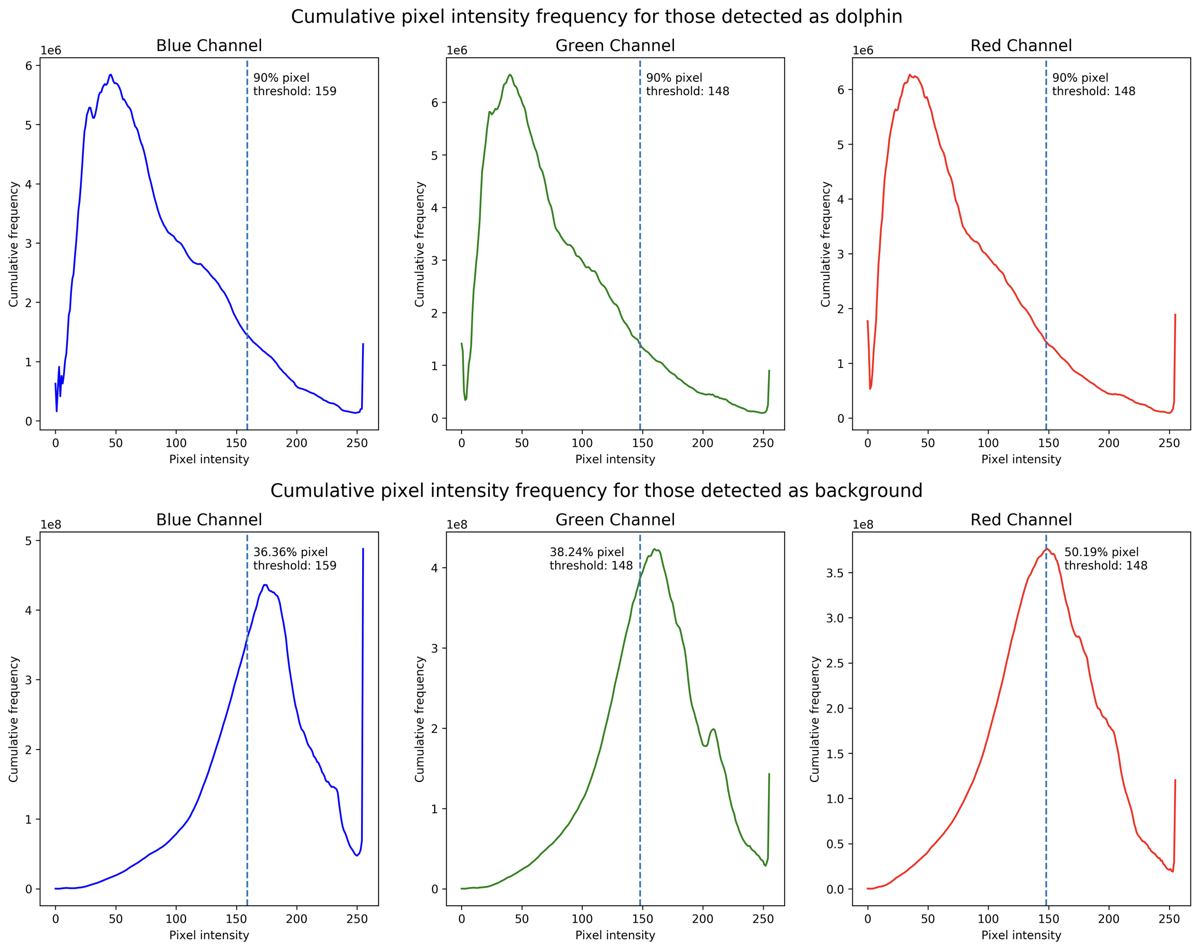
\includegraphics[scale=0.7]{Chapter5/figs/histogram-updated.png}
	\end{center}
	\caption{The global range of pixel intensities for each RGB colour channel, split by pixel classification.}\label{fig:global-histogram}
\end{figure}

Using the global distribution histograms, a \textit{dolphin-like} threshold was determined. For all masks detected as \texttt{dolphin}, 90\% of the RGB pixel intensities are below [148, 148, 159]. In contrast only 50.19\%, 38.24\%, and 36.36\% of the background pixels for each RGB channel respectively are below this threshold. As noise components in the mask are often areas of water or splash, these components will be likely much lighter in composition than cetaceans, and thus can be removed from the mask with confidence. An example of colour thresholding removing noise from a mask can be seen in Figure \ref{fig:190827-001-MOLS0078_-colour-thresholding-splash-removed}.

\begin{figure}
	\begin{center}
		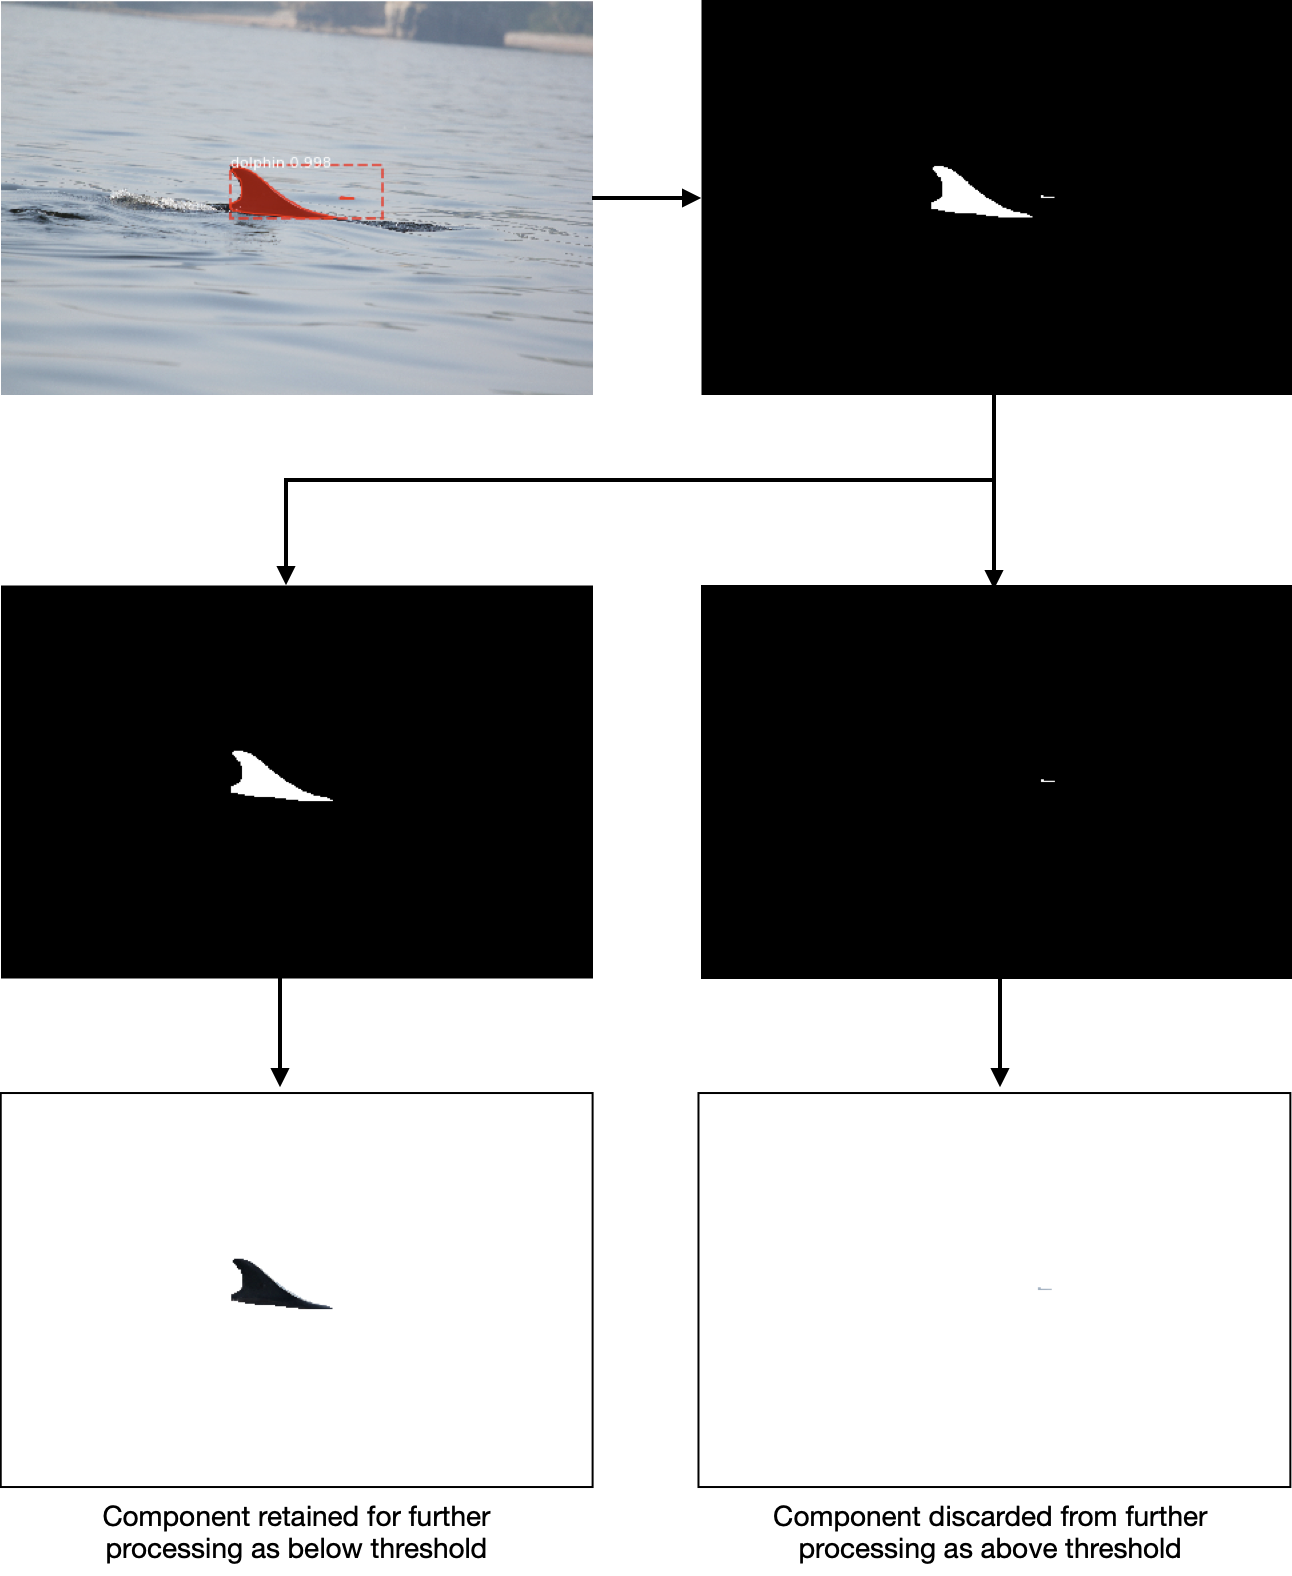
\includegraphics[scale=0.5]{Chapter5/figs/190827-001-MOLS0078_-colour-thresholding-splash-removed.png}
	\end{center}
	\caption[Workflow detailing colour thresholding to remove an area of disjoint splash which has been detected as part of a \texttt{dolphin} object.]{Workflow detailing colour thresholding to remove an area of disjoint splash which has been detected as part of a \texttt{dolphin} object. The detection mask is split into each component. The resultant background subtracted images are then colour thresholded. As a result, the erroneous splash is discarded. }\label{fig:190827-001-MOLS0078_-colour-thresholding-splash-removed}
\end{figure}

During testing however it was found that when checking detections at an individual image level rather than globally, considering a mask component to be \textit{dolphin-like} if 90\% of the pixels were below the colour threshold was too restrictive. Utilising such a high percentage bar sometimes rejected valid detections which may have been over-exposed due to lighting conditions. As such, whilst the colour threshold was kept the same, it was found that reducing the percentage check to 50\% provided enough leeway such that over-exposed but valid detections were kept whilst still rejecting a large portion of erroneous ones. Figure \ref{fig:190723-001-MOLS0752_-fin-removed-at-90-kept-at-50} shows an example detection which would be discarded if the 90\% global threshold was used per image, but is retained if this is dropped to a 50\% check.

\begin{figure}
	\begin{center}
		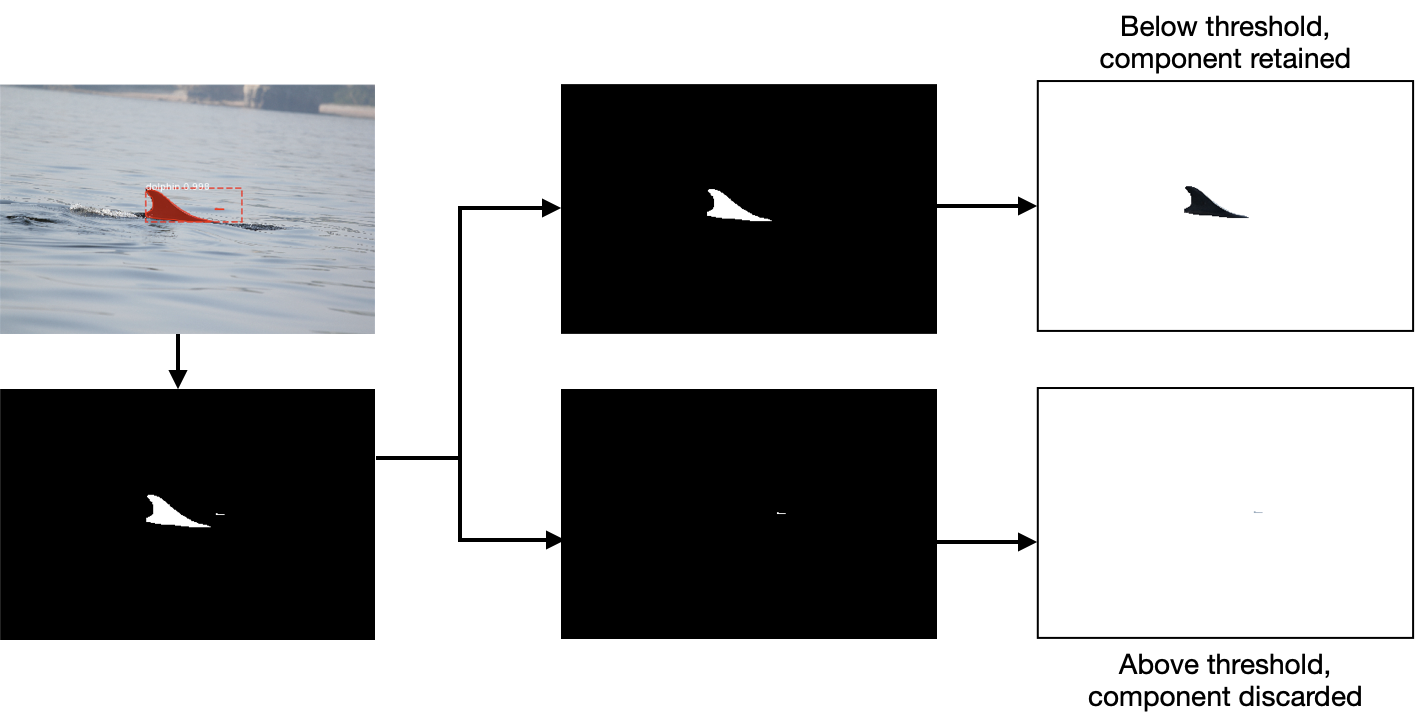
\includegraphics[width=\linewidth]{Chapter5/figs/190723-001-MOLS0752_-fin-removed-at-90-kept-at-50.png}
	\end{center}
	\caption[Workflow showing how utilising the 90\% global threshold may lead to over-exposed detections being erroneously discarded.]{Workflow showing how utilising the 90\% global threshold may lead to over-exposed detections being erroneously discarded. A \texttt{dolphin} object is detected whose mask consists of multiple components.  One of the components, which contains a valid area of detection, is shown in stage 3 of the workflow. Checking to see if 50\% of the pixels in the component are below the threshold retains the detection, whilst checking at 90\% discards it.}\label{fig:190723-001-MOLS0752_-fin-removed-at-90-kept-at-50}
\end{figure}

It may be the case that multiple components in an image meet the conditions set by the threshold to be kept. In this case, each component of the mask is split into its own image, in a similar process as outlined in Section \ref{ch:postProcessing,sec:handlingMultipleDetections}. If a mask only contains one component, then colour thresholding is not applied. This ensures no detections by the Mask R-CNN are completely ignored due to post-processing, preventing the discarding of a \texttt{dolphin} object mask which contains no disjoint components but is above the threshold, such as in the event of over-exposure. This condition also has the effect however of allowing fully erroneous detections to pass downstream, such as the flag detected in Figures \ref{fig:190730-001-MOLS0360_-detections} and \ref{fig:fin-extraction-unclean}. Any erroneous detections which pass downstream at this stage must now be handled by the identification module.

\section{Cropping}\label{ch:cetDet,sec:postProcessing,su:cropping}

At this point outputs from the Mask R-CNN detector have been post-processed to remove as much noise from the detected masks as possible, and these have been utilised to perform background subtraction. This results in an output image containing mostly white pixels surrounding a detected \texttt{dolphin} object. This image is the same size as the one inputted to the detector, which can often be many thousands of pixels, although the vast majority of these are now no longer required.

\begin{figure}
	\begin{center}
		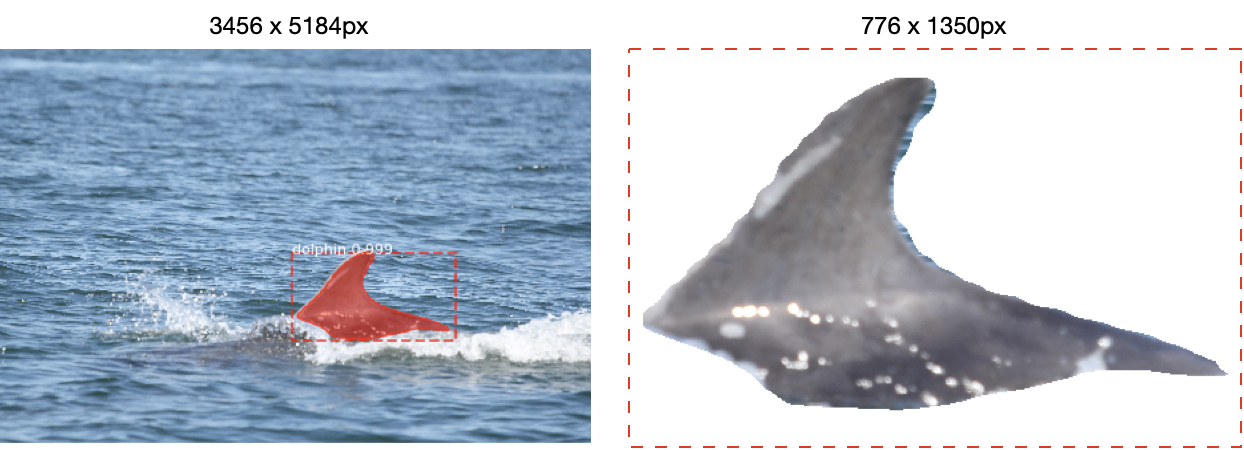
\includegraphics[scale=0.5]{Chapter5/figs/fin-extraction-unclean-updated.png}
	\end{center}
	\caption[Left: an input image and overlaid detection mask. Right: the corresponding cropped output image after post-processing.]{Left: an input image and overlaid detection mask. Right: the corresponding cropped output image after post-processing. Original image sizes are displayed above each image. Images have been resized for clarity.}\label{fig:190627-001-MOLS0028_-crop}
\end{figure}

As a result, the images outputted from the background detector are now cropped down to contain just the object of interest. This has the effect of vastly reducing the image file size, which in turn reduces the computational expense of operating on them downstream. In Figure \ref{fig:190627-001-MOLS0028_-crop} for example, the input image to the detector is of size 3456x5184 pixels. After post-processing, the resulting output image is now of size 776x1350px, approximately a 94.2\% reduction in image size whilst still keeping identifying information,  such as the white pigmentation on the dorsal fin, present. This cropping also has the effect of centring the detected \texttt{dolphin} objects in the final output image. 

\section{Post-Processing NDD20}\label{ch:postProcessing,sec:postProcessingNDD20}

NDD20 consists of large scale panoramic images, similar to the Zanzibar data before post-processing. As a result, there is a high amount of noise present in the images which should be ignored and removed before the dataset is utilised for individual identification. Whilst Chapter \ref{ch:ID} will focus on both the theory behind, and implementation of, a model capable of individual identification, this section will detail the processing of NDD20 into a form usable for the task of individual identification.

Utilising the post-processing techniques as outlined previously in this chapter, the detections from the Mask R-CNN model were used to generate a dataset of images to train another model capable of individual identification. This dataset, known as Segmented NDD20, is a collection of images which contains only the segmented masks from NDD20. 

Once images of the segmentations had been created these were then processed further to create a folder structure which allowed for easy training of an identification model. To facilitate this, each segmentation was checked against the ground truth for the image it was produced from. Any images which contained a dorsal fin with identifying information were placed in a directory containing other examples of that individual. Any fins that did not contain enough identifying information, for example due to poor segmentation such as those seen in Figure \ref{fig:removed-examples}, were removed. Whilst this removal may reduce the difficulty of the problem, as the identity of the individuals could not be confidently verified manually this also ensured mislabelling issues were not present. Noise which had passed through the mask post-processing was included in a \texttt{noise} directory with the goal of allowing any future model to learn how to identify erroneous masks that have made it through post-processing. 

\begin{figure}[b]
	\begin{center}
		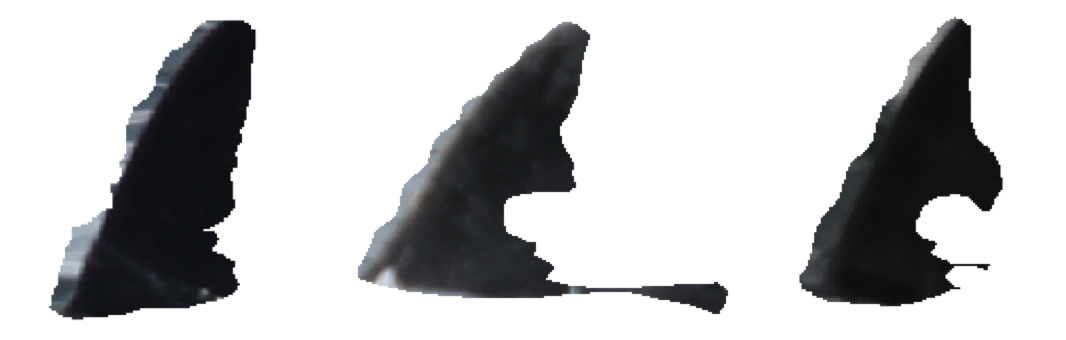
\includegraphics[scale=0.5]{Chapter5/figs/removed-segmentations.png}
	\end{center}
	\caption[Example images removed when post-processing NDD20 as their identity could not be verified manually.]{Example images removed when post-processing NDD20 as their identity could not be verified manually.}
	\label{fig:removed-examples}
\end{figure}

Example images from Segmented NDD20 are shown in Figure \ref{fig:segmented-ndd20-example}. As can be seen there is low inter-class but high intra-class differences. For example there is relatively little difference between the images shown for individuals \texttt{32} and \texttt{39}, whilst there is a large difference between the three example images for individual \texttt{11}. It is this variance and fine-grained nature which makes the task of automatic individual photo-identification particularly challenging. 

\begin{figure}
	\begin{center}
		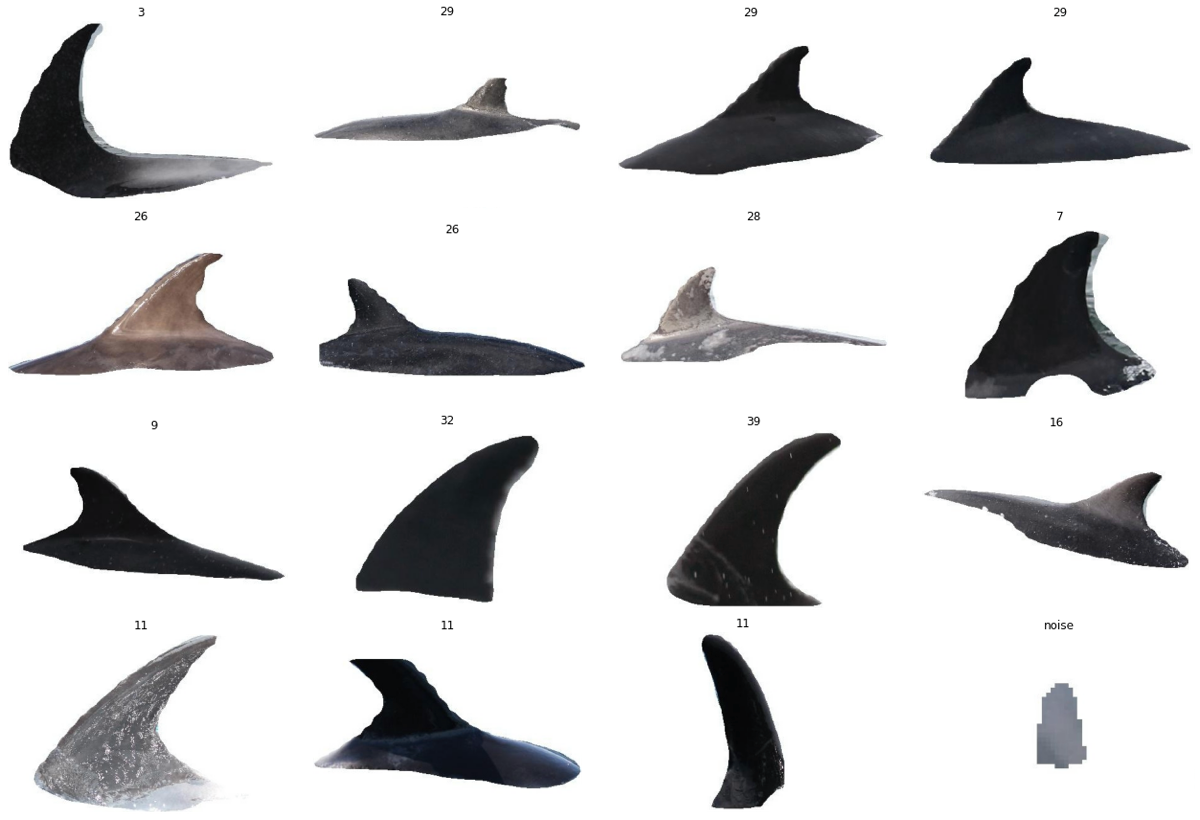
\includegraphics[scale=0.6]{Chapter5/figs/segmented-ndd20-tiled-updated.png}
	\end{center}
	\caption[Example images from Segmented NDD20.]{Example images from Segmented NDD20. The individual class label is displayed above each image.}
	\label{fig:segmented-ndd20-example}
\end{figure}

In total, Segmented NDD20 contains 1243 images representing 43 classes including \texttt{noise}. Individuals \texttt{6} and \texttt{27} were removed from the dataset by the post-processing algorithm. Upon examination, images of these individuals were captured from extreme angles or with large amounts of splash, making it difficult for the detector to produce accurate segmentations. The dataset is highly skewed with approximately 66\% of images in the dataset labelled as \texttt{noise}. Classes representing individual animals contain a non-uniform number of example images (median = 8.5) varying between 33 examples for individual \texttt{11} to just one for individuals \texttt{5} and \texttt{35}. As such this dataset represents not just a fine-grained but also a few-shot problem, a combination which is extremely challenging for current computer vision methods. 

\subsection{Additional External Data}\label{ch:postProcessing,sec:NDD_AU_SMRU}

After post-processing the data collected during fieldwork into the Segmented NDD20 dataset, it was clear from the class distribution present that it may be beneficial to increase the number of examples per individual, providing a photo-id model more data to learn from. As it was not possible due to sea state conditions to continue data collection in the Coquet to St. Mary's MCZ after 10/10/2019, work was undertaken to procure data from other external sources. 

As a result of the large range traversed by cetaceans \cite{shane_ecology_1986} there was a chance that the individuals catalogued in the MCZ had also been recorded in other areas. The underwater habitat found in the MCZ extends upwards as far as the Moray Firth in Scotland. This, along with the knowledge the animals prefer colder waters, led to the assumption that the animals found in Northumberland would likely also be found in catalogues maintained further north. Examination of photo-id catalogues from the University of Aberdeen, provided after discussions with the manager of the University's long-term bottlenose dolphin studies Dr. Barbara Cheney, confirmed a catalogue overlap. It was determined that 23 individuals (all bottlenose dolphins) were present in both catalogues. As a result of this analysis, Dr. Cheney provided 1827 additional images of the overlapping individuals to complement Segmented NDD20. Images provided were collected by both the University of Aberdeen and the University of St. Andrews' Sea Mammal Research Unit (SMRU)\nomenclature[z-SMRU]{SMRU}{Sea Mammal Research Unit} with the approval of Dr. M\`{o}nica Arso Civil. These images were captured during surveys undertaken between 2003-2019 and were of the highest quality rating on the scale used by the institutions. All images contained only a single individual. 

The additional external data procured was passed through the Mask R-CNN detector and post-processing algorithm, producing images similar to those already present in Segmented NDD20. The post-processed Aberdeen and SMRU data was combined with Segmented NDD20 to produce the NDD AU SMRU dataset, consisting of 2626 images (1383 more than Segmented NDD20) representing 44 classes including \texttt{noise}. Individual \texttt{6}, whilst not present in Segmented NDD20 is accounted for in NDD AU SMRU, however individual \texttt{27} still remains absent. Like Segmented NDD20, NDD AU SMRU is heavily skewed towards \texttt{noise} with 61\% of images labelled as this class. Non-\texttt{noise} classes however now have a median of 22 examples per class, providing a larger number of example images to train an automatic photo-id model from. 

\section{Summary}\label{ch:postProcessing,sec:summary}

This chapter discusses the creation of a post-processing methodology for dorsal fin detections generated by the Mask R-CNN model as outlined in Chapter \ref{ch:cetDet}. The model's outputted detections are coupled with post-processing techniques capable of greatly reducing the amount, and improving the quality of, data on which subcomponents further into the system pipeline are required to operate. Whilst no quantification of the post-processing methodology is undertaken, the inclusion of these stages in the pipeline allows for greater computational efficiency downstream as well as more accurate individual identifications. 

The developed post-processing methodology is then utilised for the creation of Segmented NDD20, a dataset to be utilised for the training of a neural network capable of individual identification. Finally, the NDD AU SMRU dataset is created by combining Segmented NDD20 and additional data provided by collaborators at the Universities of Aberdeen and St. Andrews after a cross-catalogue matching process was undertaken, highlighting a 23 individual overlap between the catalogues maintained by Newcastle University and the two collaborating universities. A comparison between the NDD20, Segmented NDD20, and NDD AU SMRU datasets is provided in Table \ref{tab:ndd-dataset-overview}.

\begin{table}[]
	
	\begin{tabular}{ccccc}
		\hline
		\textbf{Dataset}             & \textbf{\begin{tabular}[c]{@{}c@{}}Number\\ of Images\end{tabular}} & \textbf{\begin{tabular}[c]{@{}c@{}}Number\\ of Individuals\end{tabular}} & \textbf{\begin{tabular}[c]{@{}c@{}}Noise Class\\ Included?\end{tabular}} & \textbf{\begin{tabular}[c]{@{}c@{}}Total Number\\ of Classes\end{tabular}} \\ \hline
		\textbf{NDD20 (Above Water)} & 2201                                                                & 44                                                                       & \xmark                                                                   & 44                                                                         \\
		\textbf{NDD20 (Below Water)} & 2201                                                                & 82                                                                       & \xmark                                                                   & 82                                                                         \\
		\textbf{Segmented NDD20}     & 1243                                                                & 42                                                                       & \cmark                                                                   & 43                                                                         \\
		\textbf{NDD AU SMRU}         & 2626                                                                & 43                                                                       & \cmark                                                                   & 44                                                                         \\ \hline
	\end{tabular}
	\caption{A comparison between the NDD20, Segmented NDD20, and NDD AU SMRU datasets.}
	\label{tab:ndd-dataset-overview}
\end{table}

Masks post-processed by the methodology outlined within this chapter are then passed to the next stage of the system pipeline, consisting of a model trained to perform accurate most likely catalogue matching. This model is examined in detail in Chapter \ref{ch:ID}. 
